\documentclass[12pt, a4paper]{scrartcl}

\usepackage{ucs}
\usepackage[utf8x]{inputenc}
\usepackage[T1]{fontenc}
\usepackage{amsmath,amssymb,amstext}
\usepackage{graphicx}
\usepackage{textgreek}
\usepackage{framed,xcolor}
\usepackage[format=hang,indention=-1.2cm,font=footnotesize]{caption}
\usepackage{soul}
\setlength{\parindent}{0.5cm} 
\setlength{\parskip}{0.35cm}
\usepackage{setspace}
\usepackage{float}
\usepackage[numbib]{tocbibind}
\usepackage{sectsty}
\usepackage{enumitem}
\sectionfont{\Large}
\subsectionfont{\large}

\usepackage{geometry}
\geometry{a4paper, top=2.88cm, bottom=3.5cm, left=2cm, right=2cm}

\usepackage{enumitem}
\usepackage{hyperref}
\usepackage{courier}
\usepackage{listings}
\lstset{basicstyle=\footnotesize\ttfamily}

\author{David Kleindienst}
\title{Automatic imaging with serialEM and synapseFinder}
\begin{document}
\maketitle
\section{Introduction}

\section{The SerialEM Interface}
\begin{figure}[H]
\includegraphics[width=\linewidth]{screenshots/serEM.png}
\caption[SerialEM Interface]{Text here}
\end{figure}

\section{Take an overview image of the whole replica}

\begin{figure}[H]
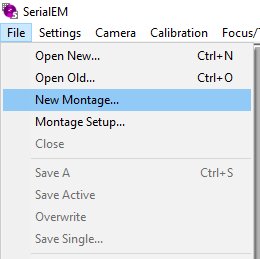
\includegraphics[width=\linewidth]{screenshots/NewMontage.png}
\caption{NewMontage}
\end{figure}

\begin{figure}[H]
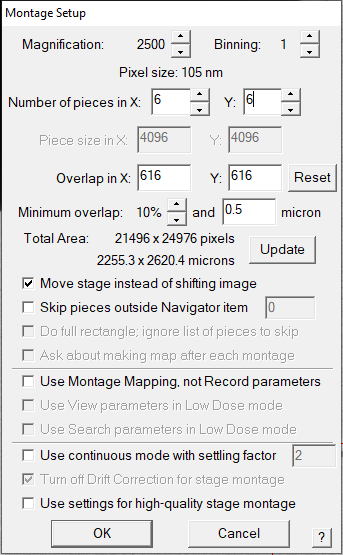
\includegraphics[scale=1]{screenshots/OverviewSetup1.png}
\caption{Text}
\end{figure}

\begin{figure}[H]
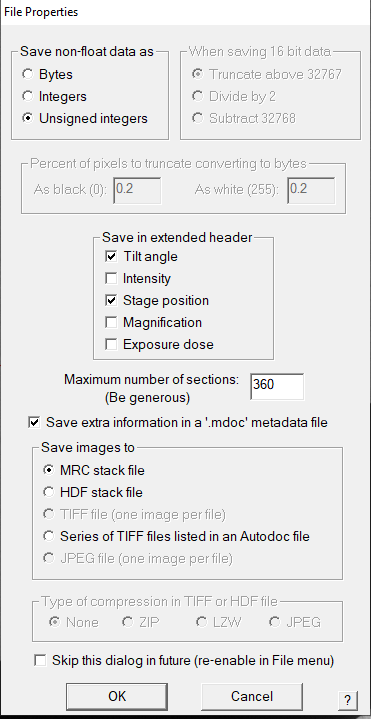
\includegraphics[scale=1]{screenshots/OverviewSetup2.png}
\caption{Text}
\end{figure}

\begin{figure}[H]
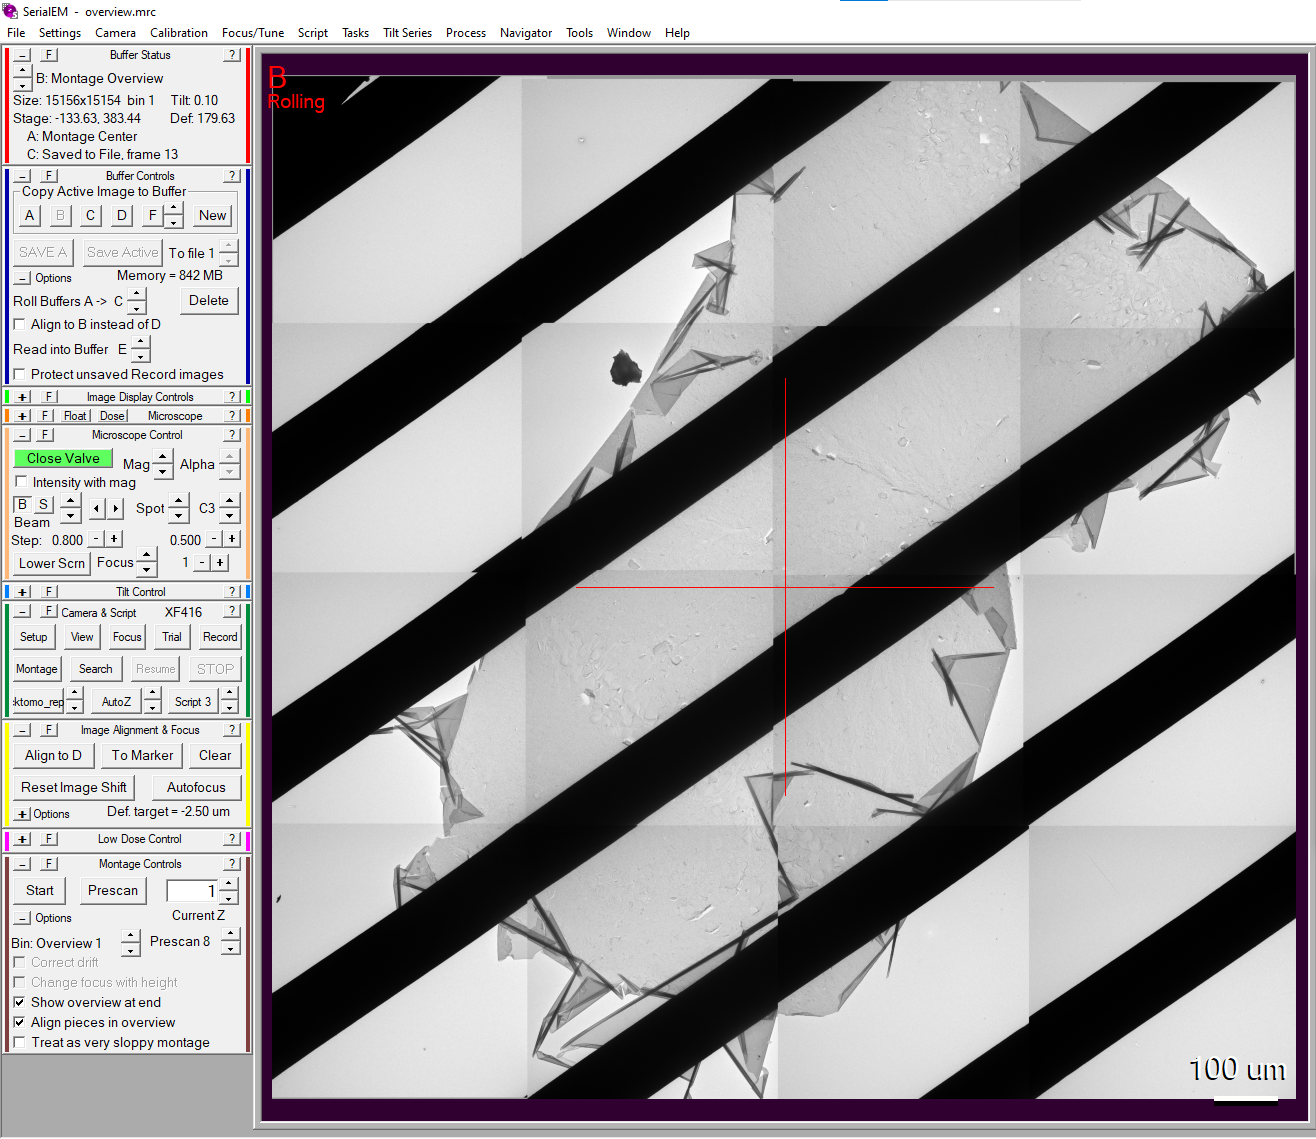
\includegraphics[width=\linewidth]{screenshots/Overview.png}
\caption{Text}
\end{figure}



\section{Make overview a map and align with higher mag}


\begin{figure}[H]
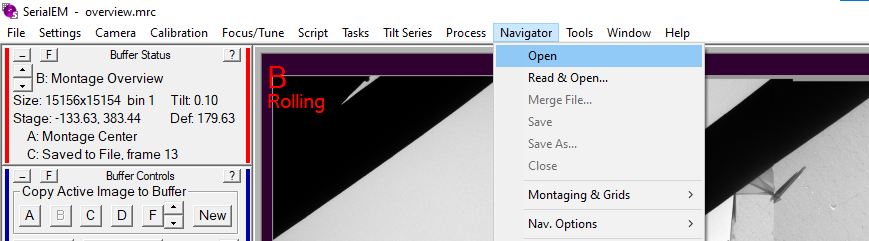
\includegraphics[width=\linewidth]{screenshots/OpenNavigator.png}
\caption{Text}
\end{figure}


\begin{figure}[H]
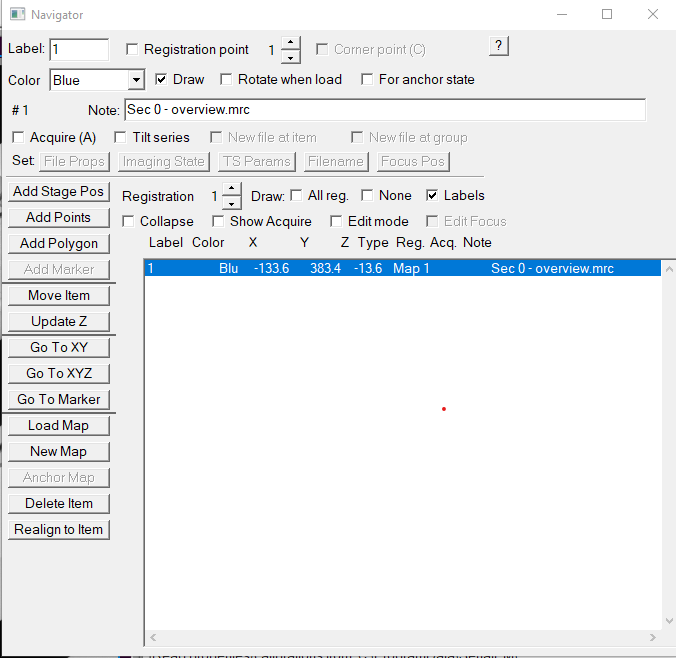
\includegraphics[scale=1]{screenshots/Navigator_addOverview.png}
\caption{Text}
\end{figure}

\begin{figure}[H]
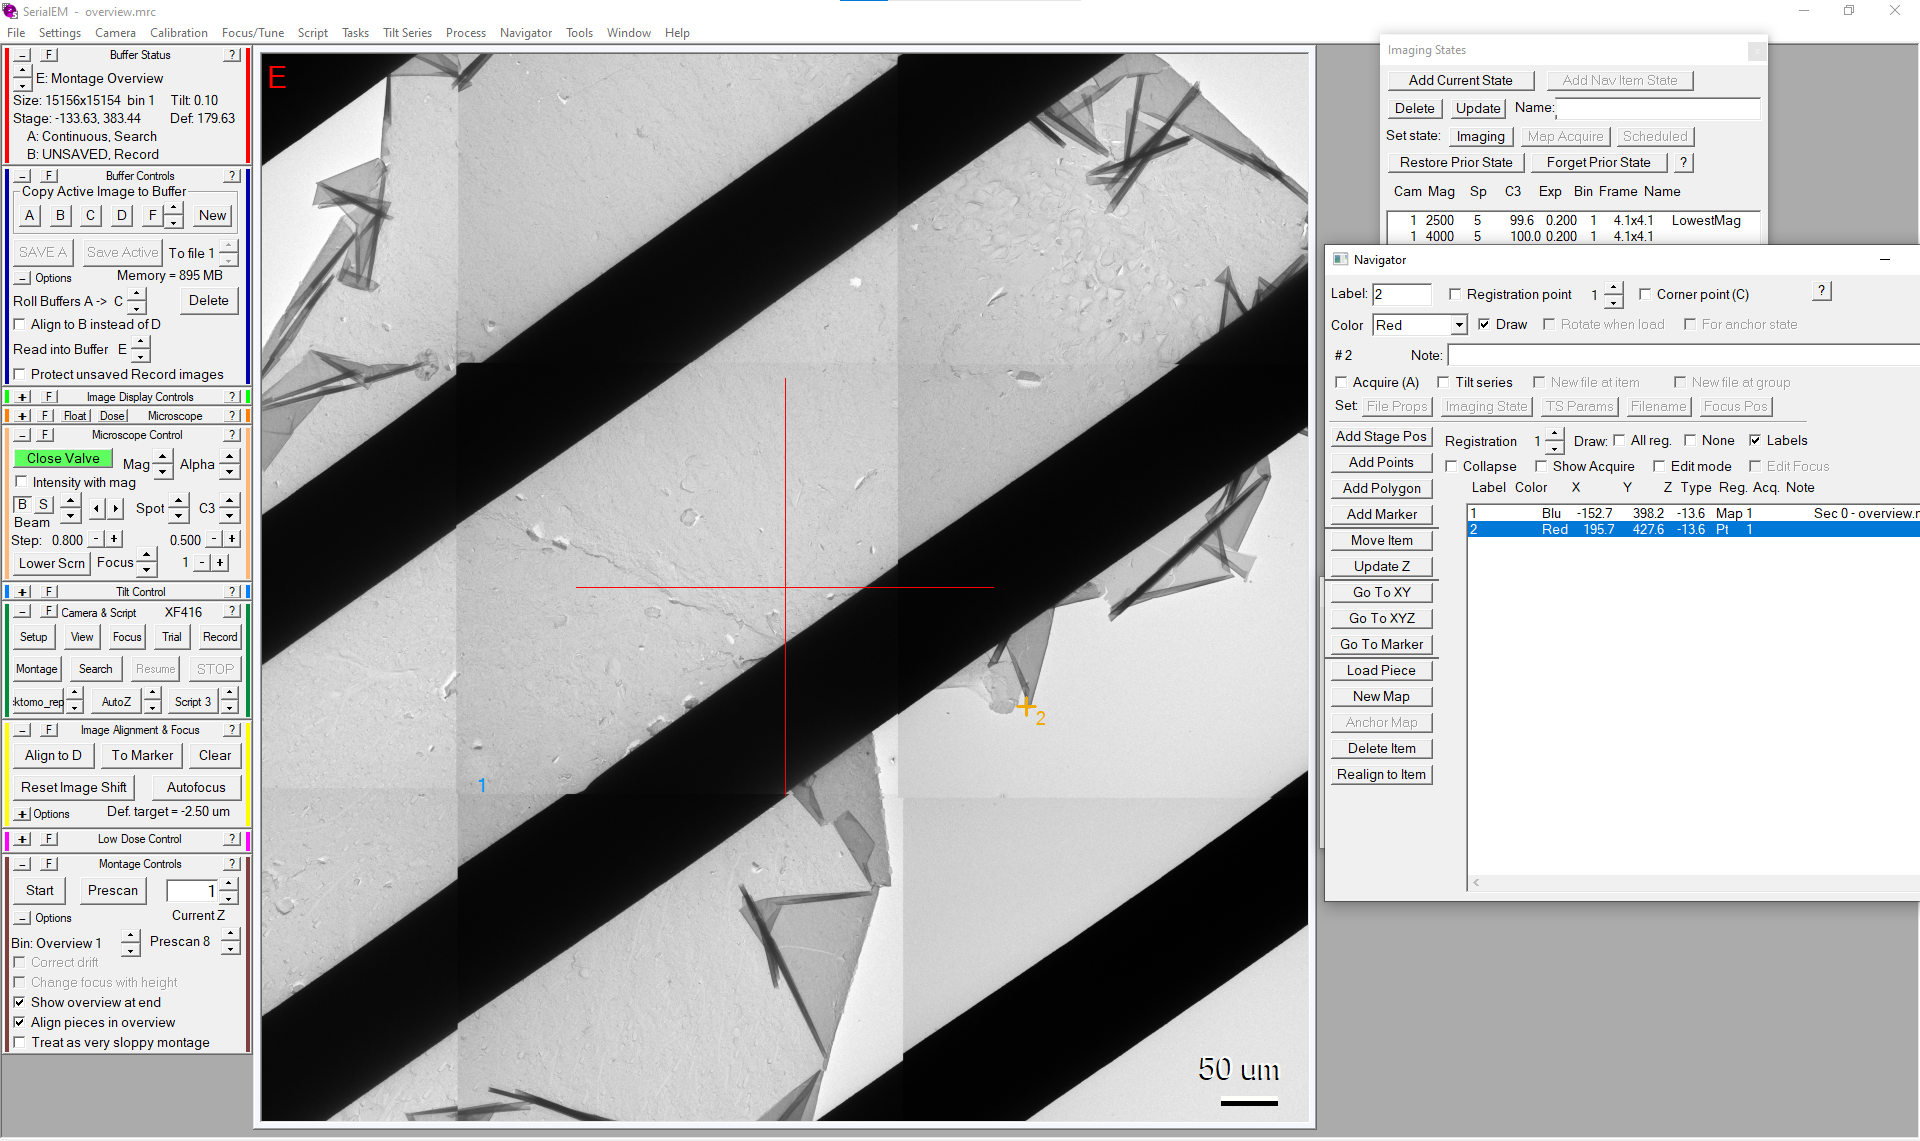
\includegraphics[width=\linewidth]{screenshots/PointOnLandmark.png}
\caption{Text}
\end{figure}

\begin{figure}[H]
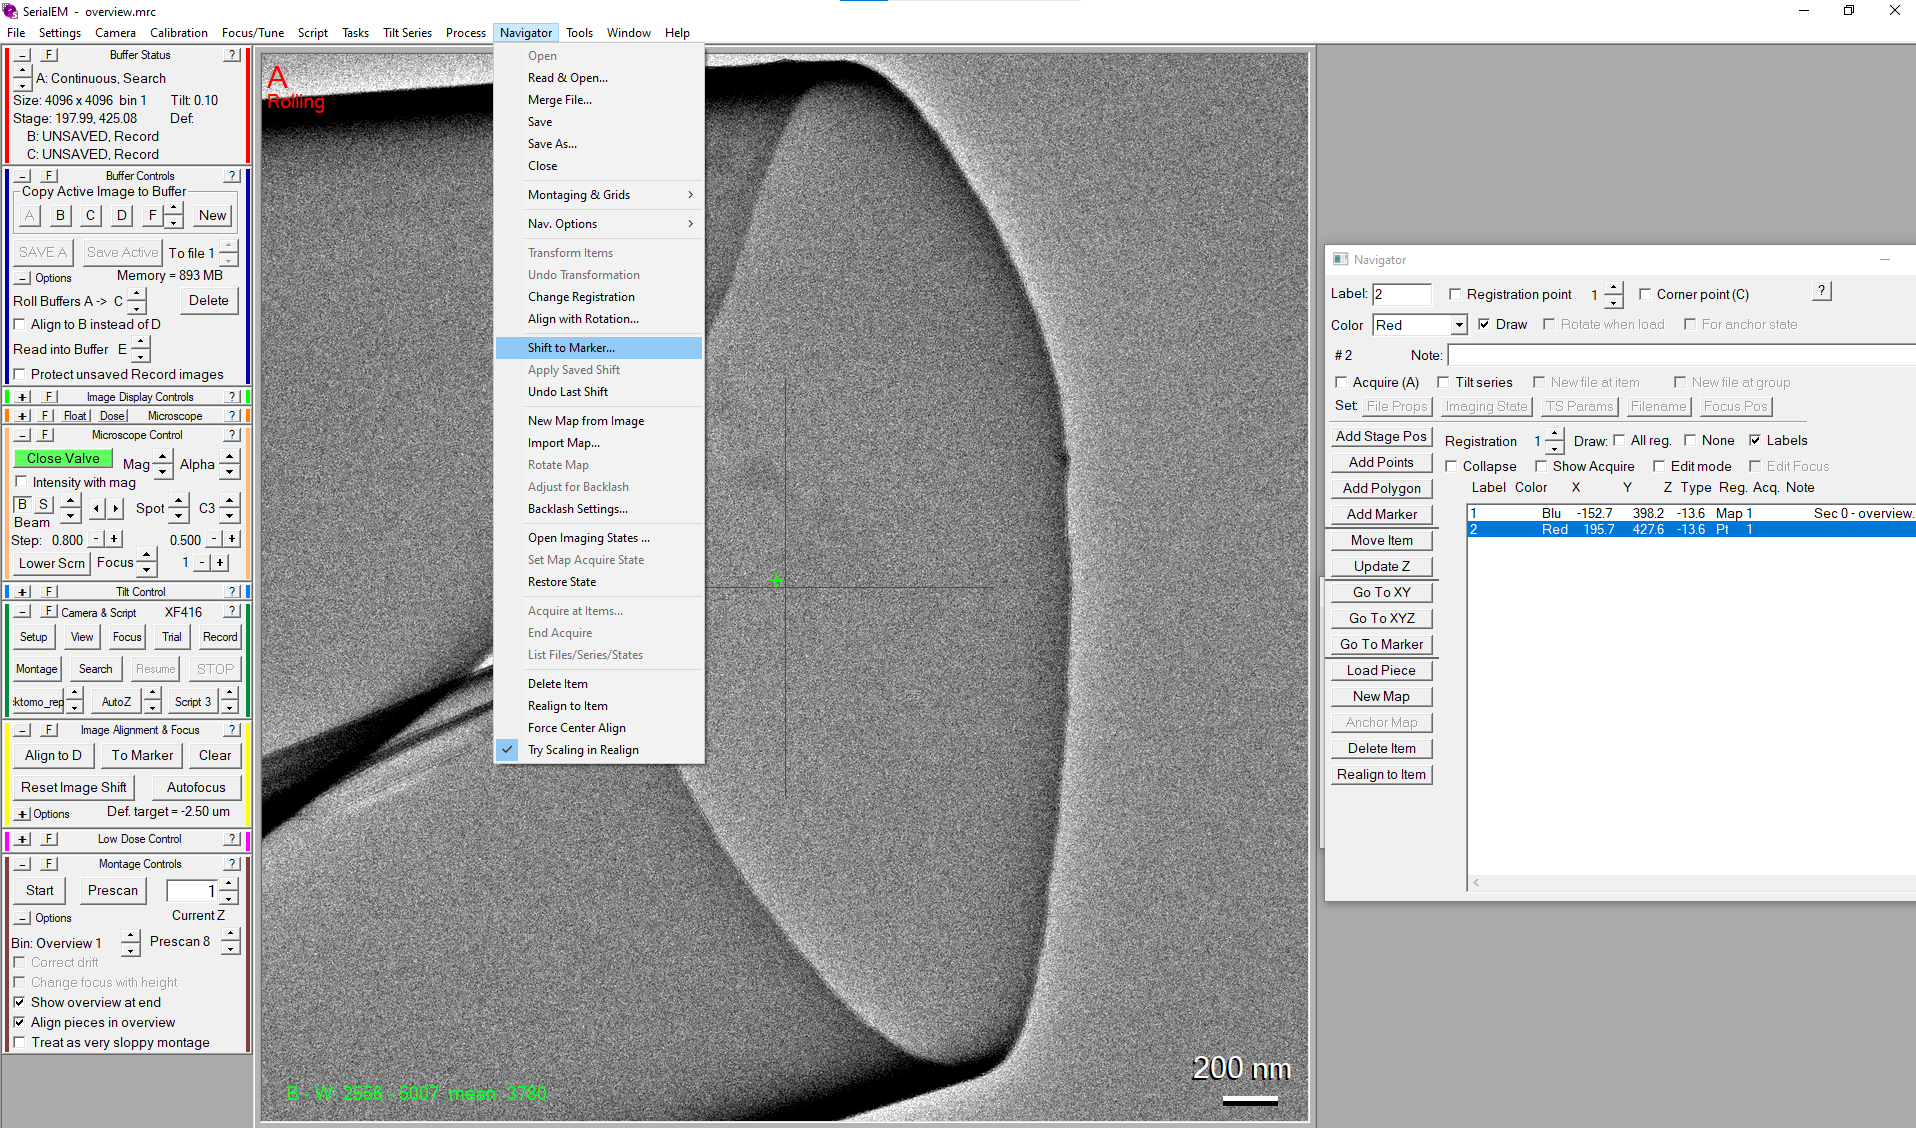
\includegraphics[width=\linewidth]{screenshots/PointOnLandmarkZoom.png}
\caption{Text}
\end{figure}

\begin{figure}[H]
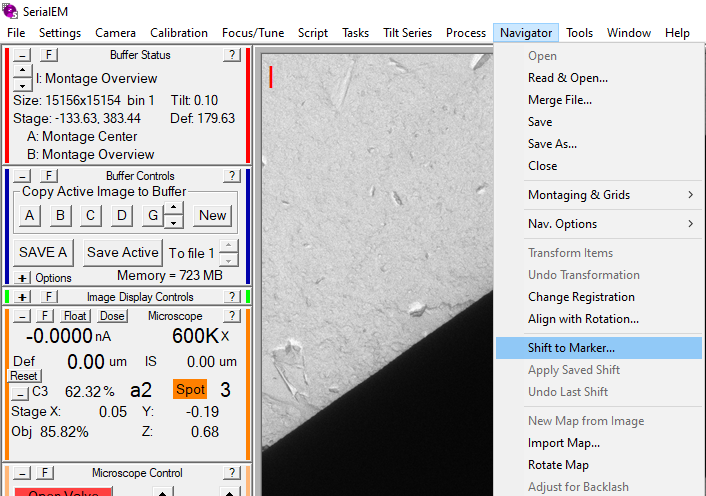
\includegraphics[width=\linewidth]{screenshots/ShiftToMarker.png}
\caption{Text}
\end{figure}

\begin{figure}[H]
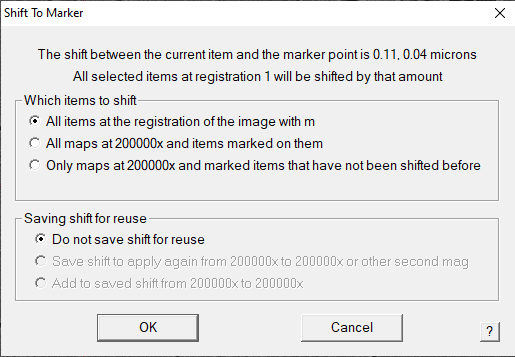
\includegraphics[width=\linewidth]{screenshots/ShiftToMarkerMapMenu.png}
\caption{Text}
\end{figure}

\section{Take intermediate magnification image of your region of interest}

\begin{figure}[H]
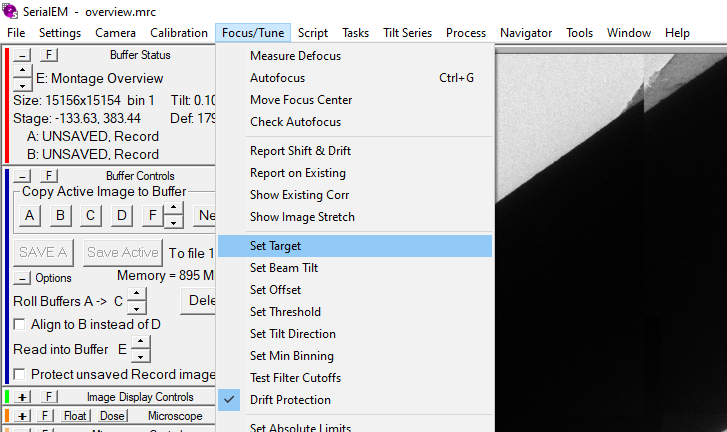
\includegraphics[width=\linewidth]{screenshots/TargetDefocus.png}
\caption{Text}
\end{figure}

\begin{figure}[H]
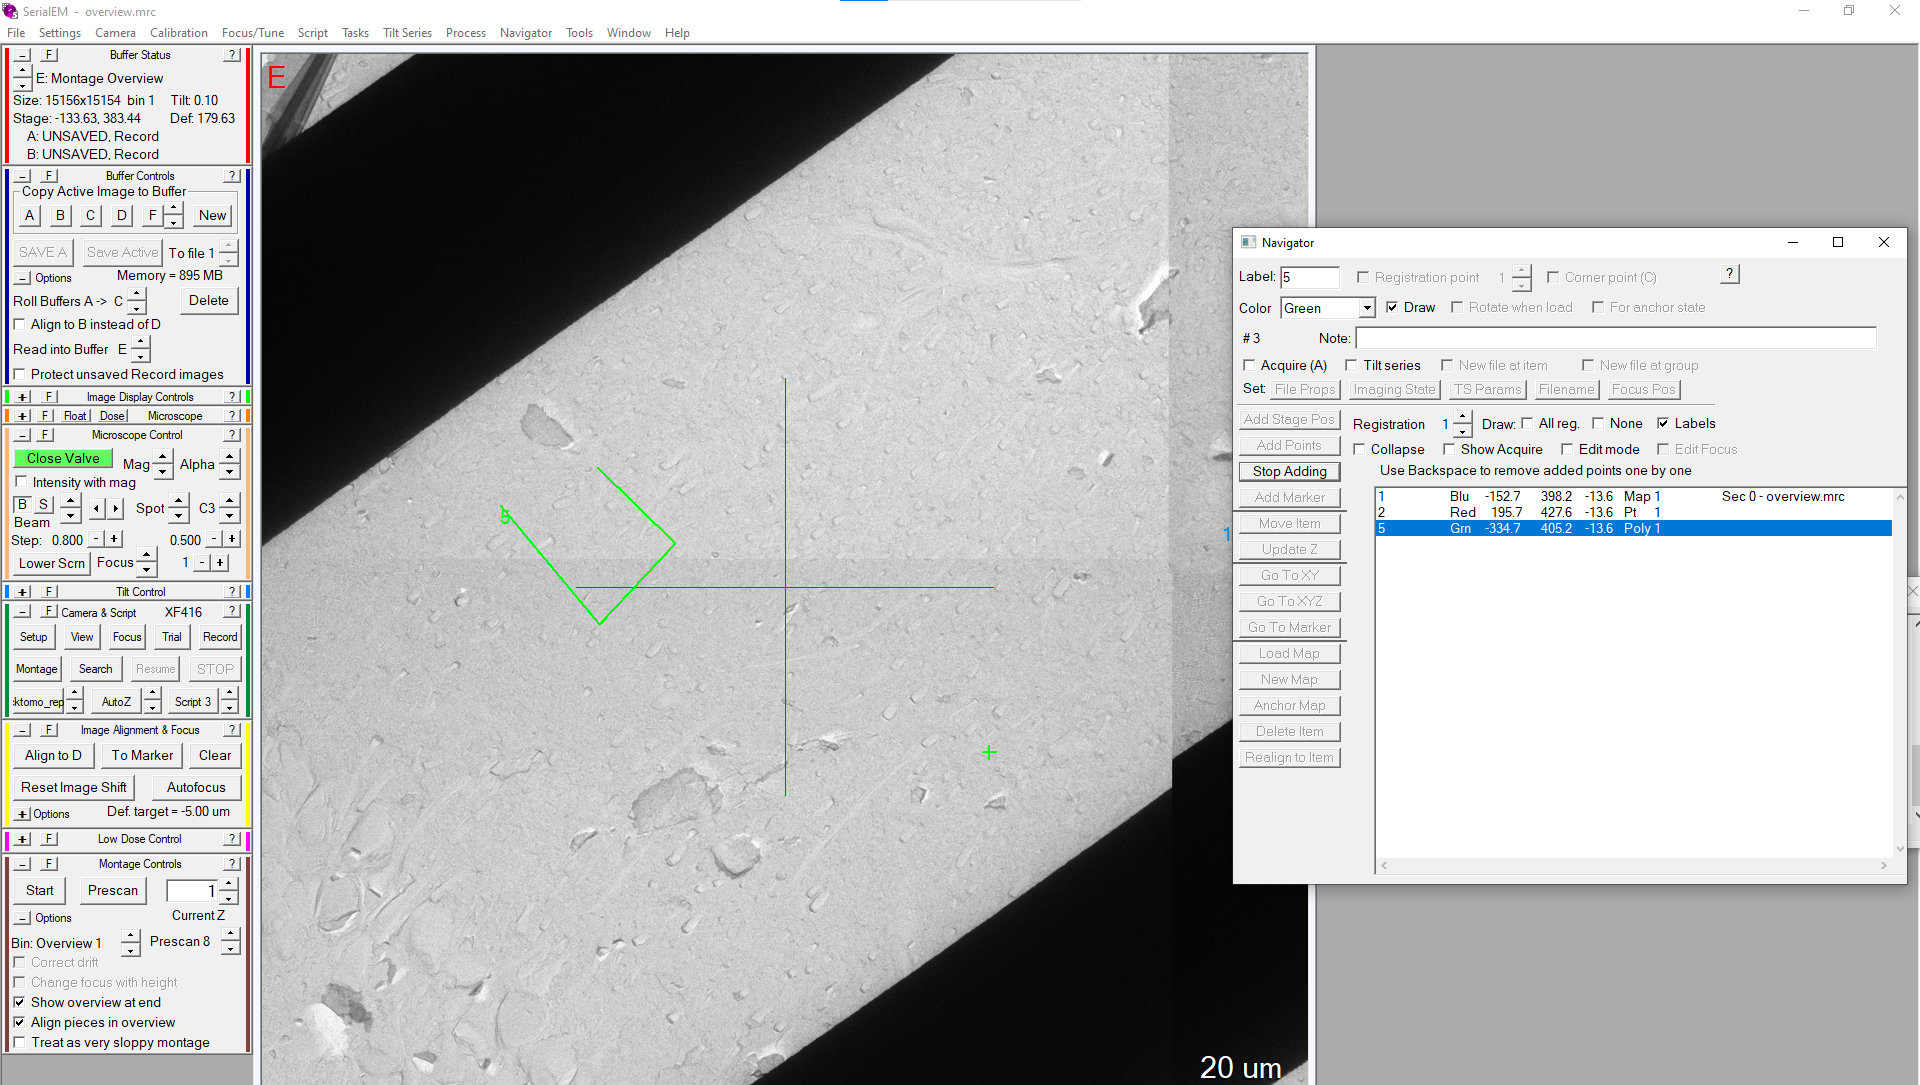
\includegraphics[width=\linewidth]{screenshots/AddPolygon.png}
\caption{Text}
\end{figure}

\begin{figure}[H]
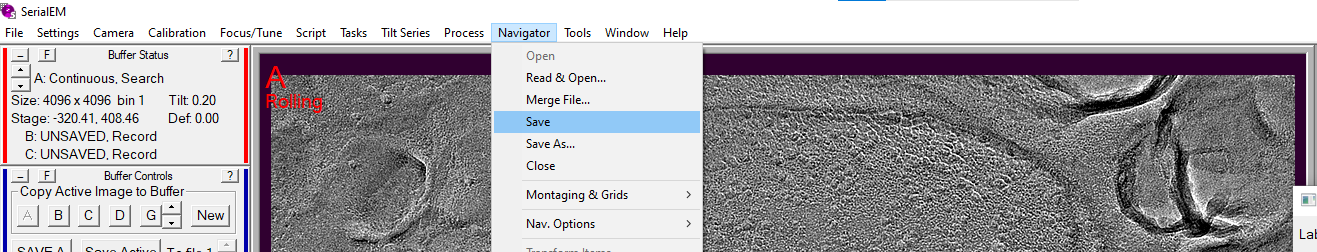
\includegraphics[width=\linewidth]{screenshots/NavigatorSave.png}
\caption{This file should be saved in the same folder as your images}
\end{figure}

\begin{figure}[H]
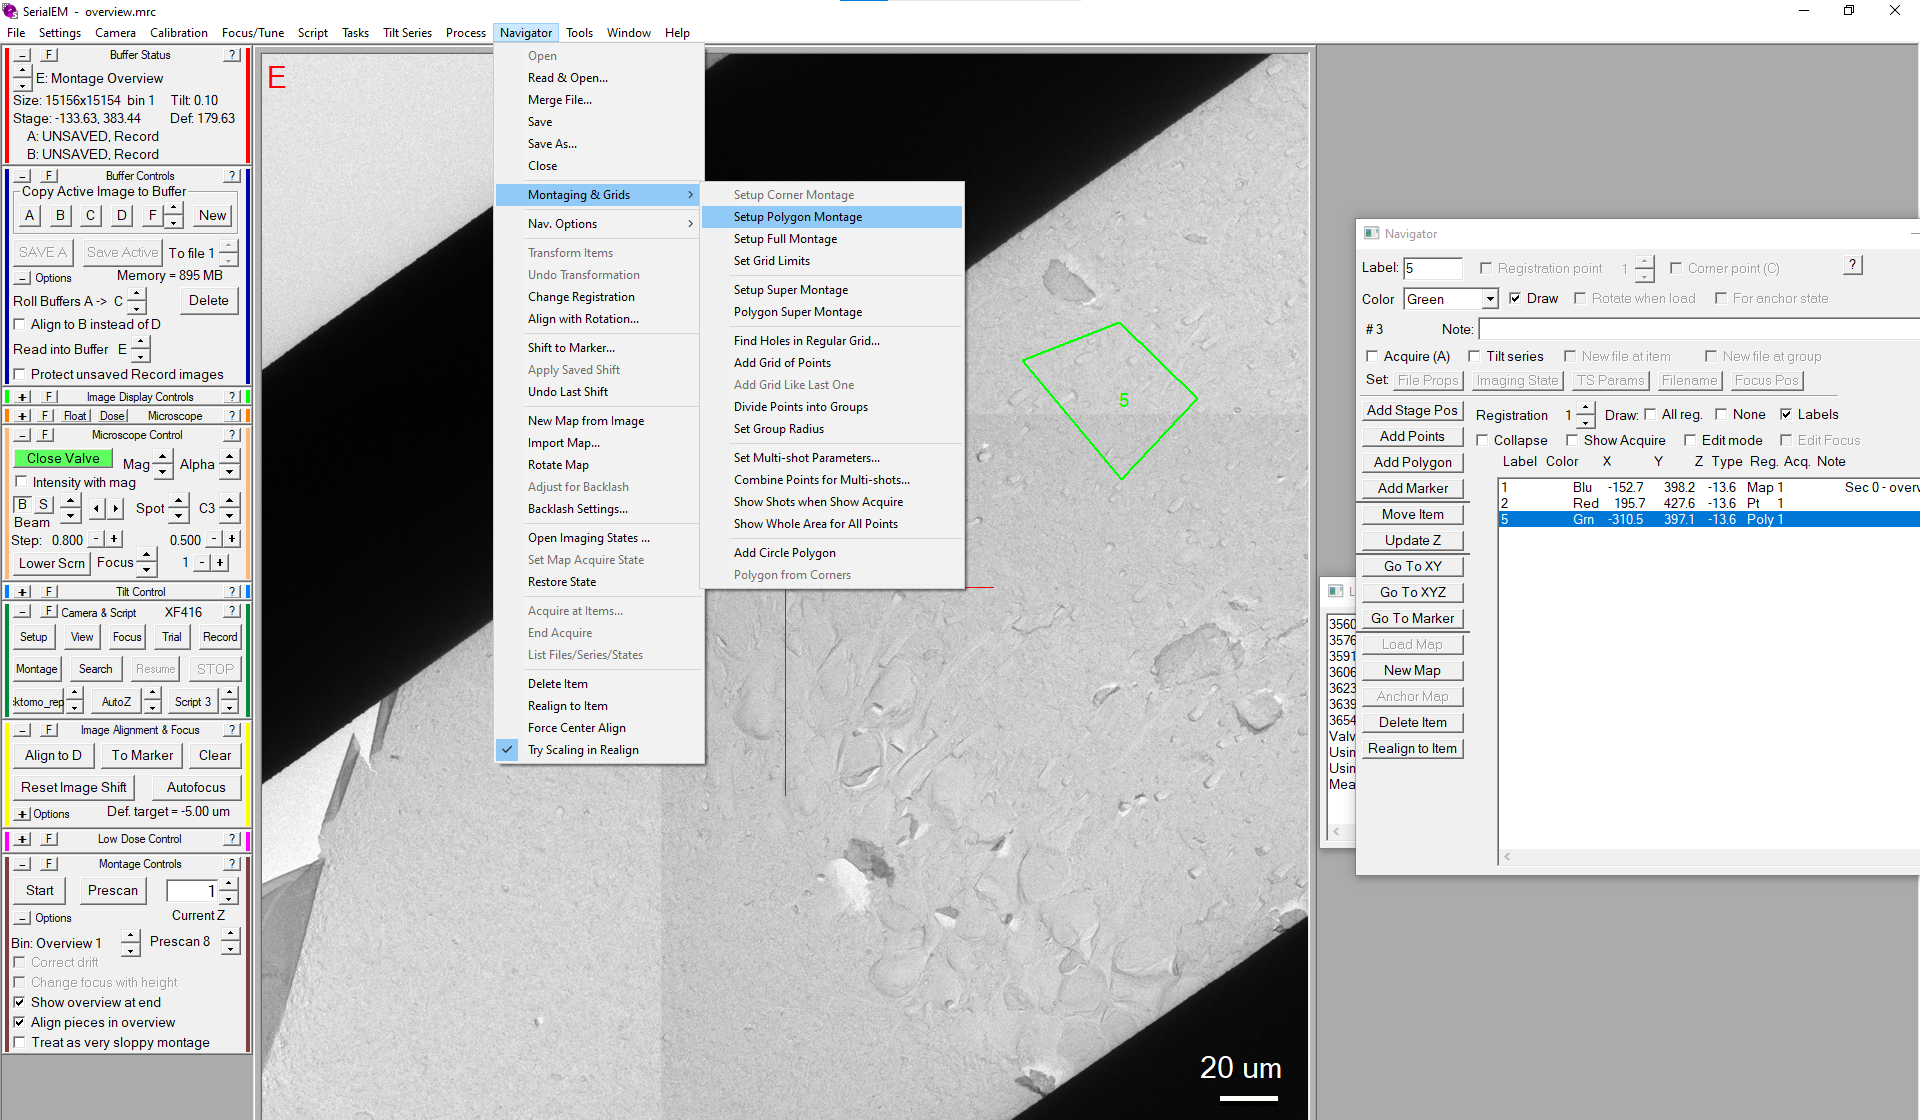
\includegraphics[width=\linewidth]{screenshots/SetupPolygonMontage.png}
\caption{Text}
\end{figure}

\begin{figure}[H]
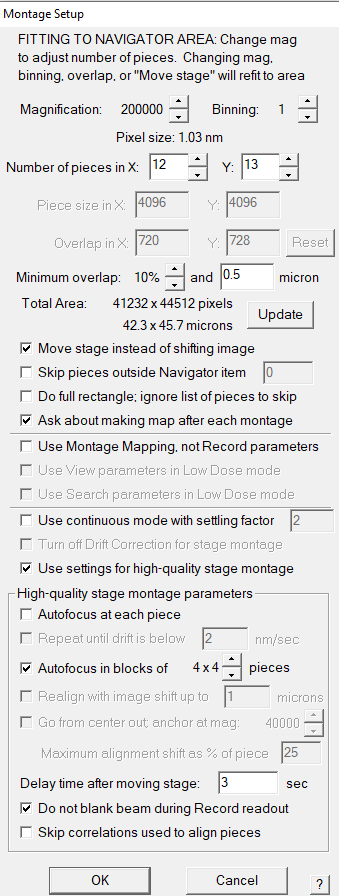
\includegraphics[scale=1]{screenshots/SetupPolygonMontage2.png}
\caption{Text}
\end{figure}

\begin{figure}[H]
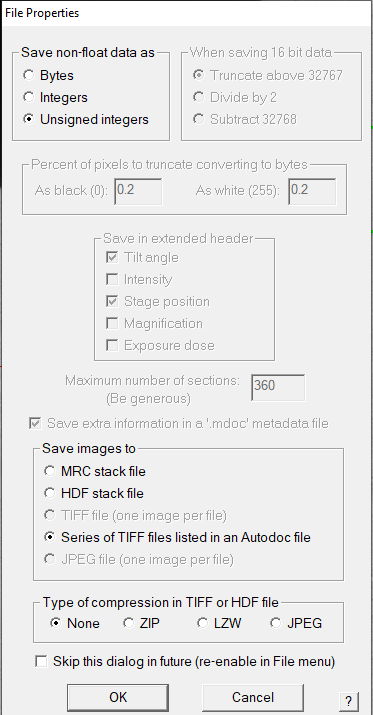
\includegraphics[scale=1]{screenshots/SetupPolygonMontage3.png}
\caption{Text}
\end{figure}


\begin{figure}[H]
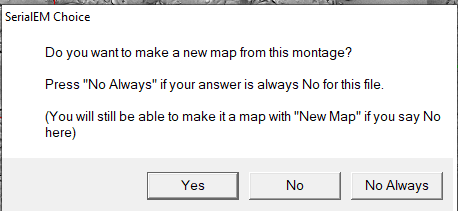
\includegraphics[scale=1]{screenshots/AddAsMap.png}
\caption{Text}
\end{figure}


\section{Automatically find the features of interest - Using the GPU on the microscope PC}


\begin{figure}[H]
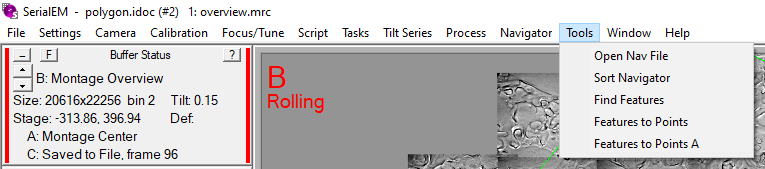
\includegraphics[width=\linewidth]{screenshots/Tools.png}
\caption{Text}
\end{figure}

\begin{figure}[H]
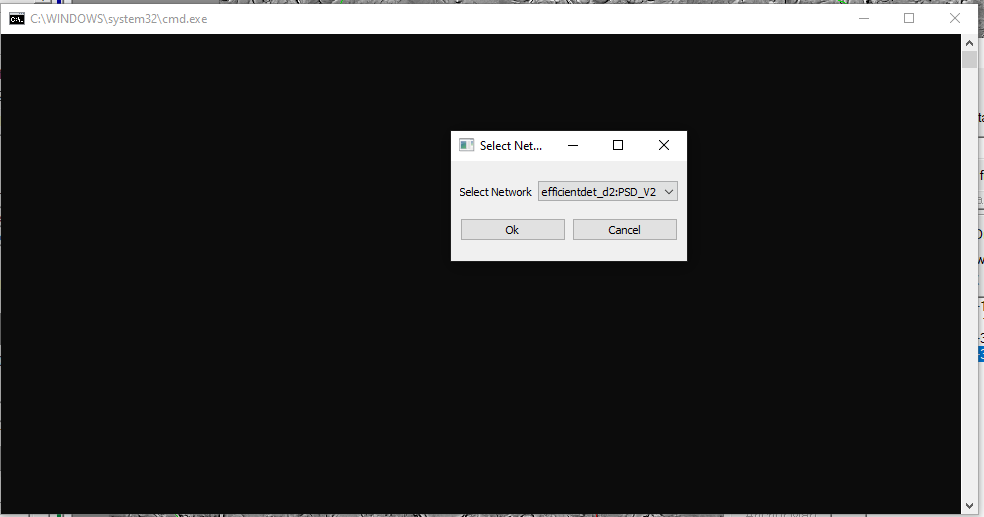
\includegraphics[width=\linewidth]{screenshots/FindFeatures.png}
\caption{Text}
\end{figure}

\section{Automatically find the features of interest - Using another PC with access to the same network drive}

This can be done at the same time as the microscope is imaging

\subsection{Windows}

\begin{figure}[H]
\includegraphics[width=\linewidth]{screenshots/serEMSynapsePredictCmd.png}
\caption{Text}
\end{figure}

\begin{figure}[H]
\includegraphics[width=\linewidth]{screenshots/serEMSynapseFinderMenu.png}
\caption{Text}
\end{figure}


\section{Add detections to the map}

\begin{figure}[H]
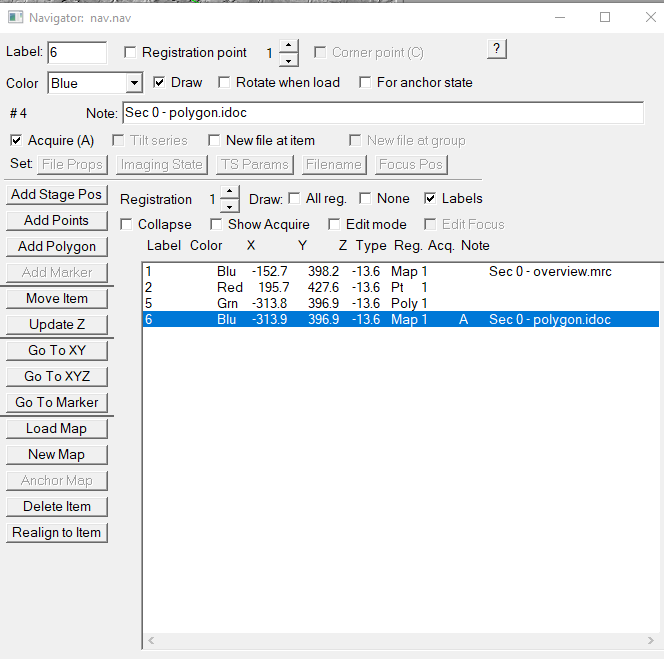
\includegraphics[scale=1]{screenshots/NavigatorAcquireMap.png}
\caption{Text}
\end{figure}

\begin{figure}[H]
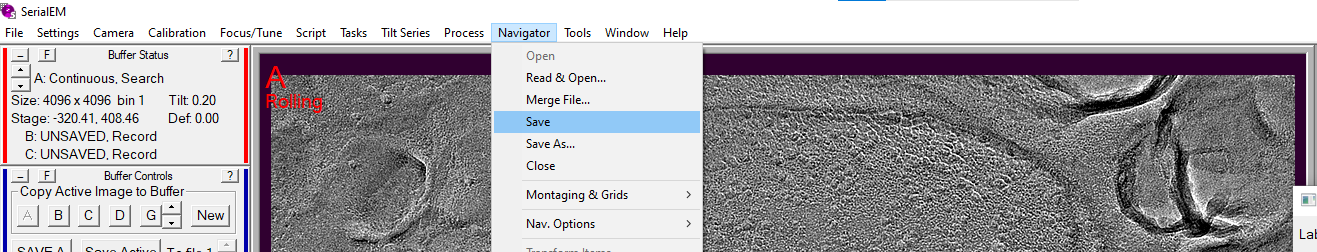
\includegraphics[width=\linewidth]{screenshots/NavigatorSave.png}
\caption{Text}
\end{figure}

\begin{figure}[H]
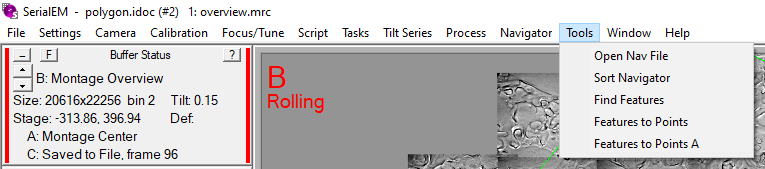
\includegraphics[width=\linewidth]{screenshots/Tools.png}
\caption{Text}
\end{figure}

\begin{figure}[H]
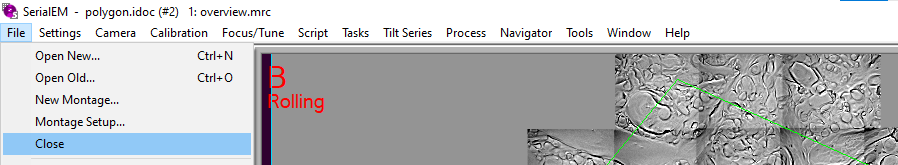
\includegraphics[width=\linewidth]{screenshots/File_Close.png}
\caption{Text}
\end{figure}

\begin{figure}[H]
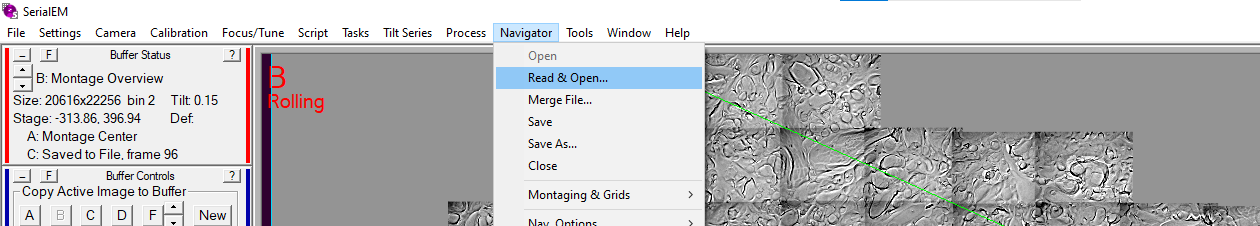
\includegraphics[width=\linewidth]{screenshots/NavigatorReadAndOpen.png}
\caption{Text}
\end{figure}


\begin{figure}[H]
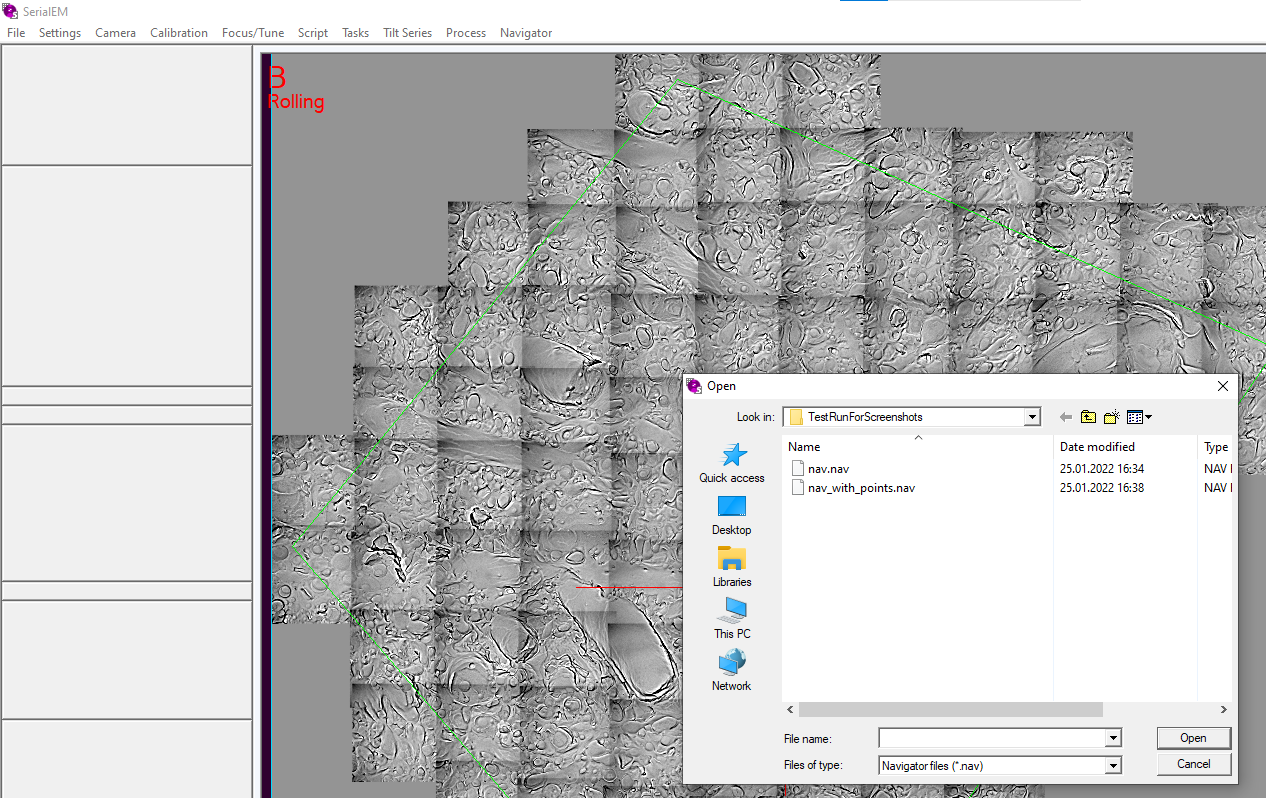
\includegraphics[width=\linewidth]{screenshots/OpenNavWithPoints.png}
\caption{Text}
\end{figure}

\begin{figure}[H]
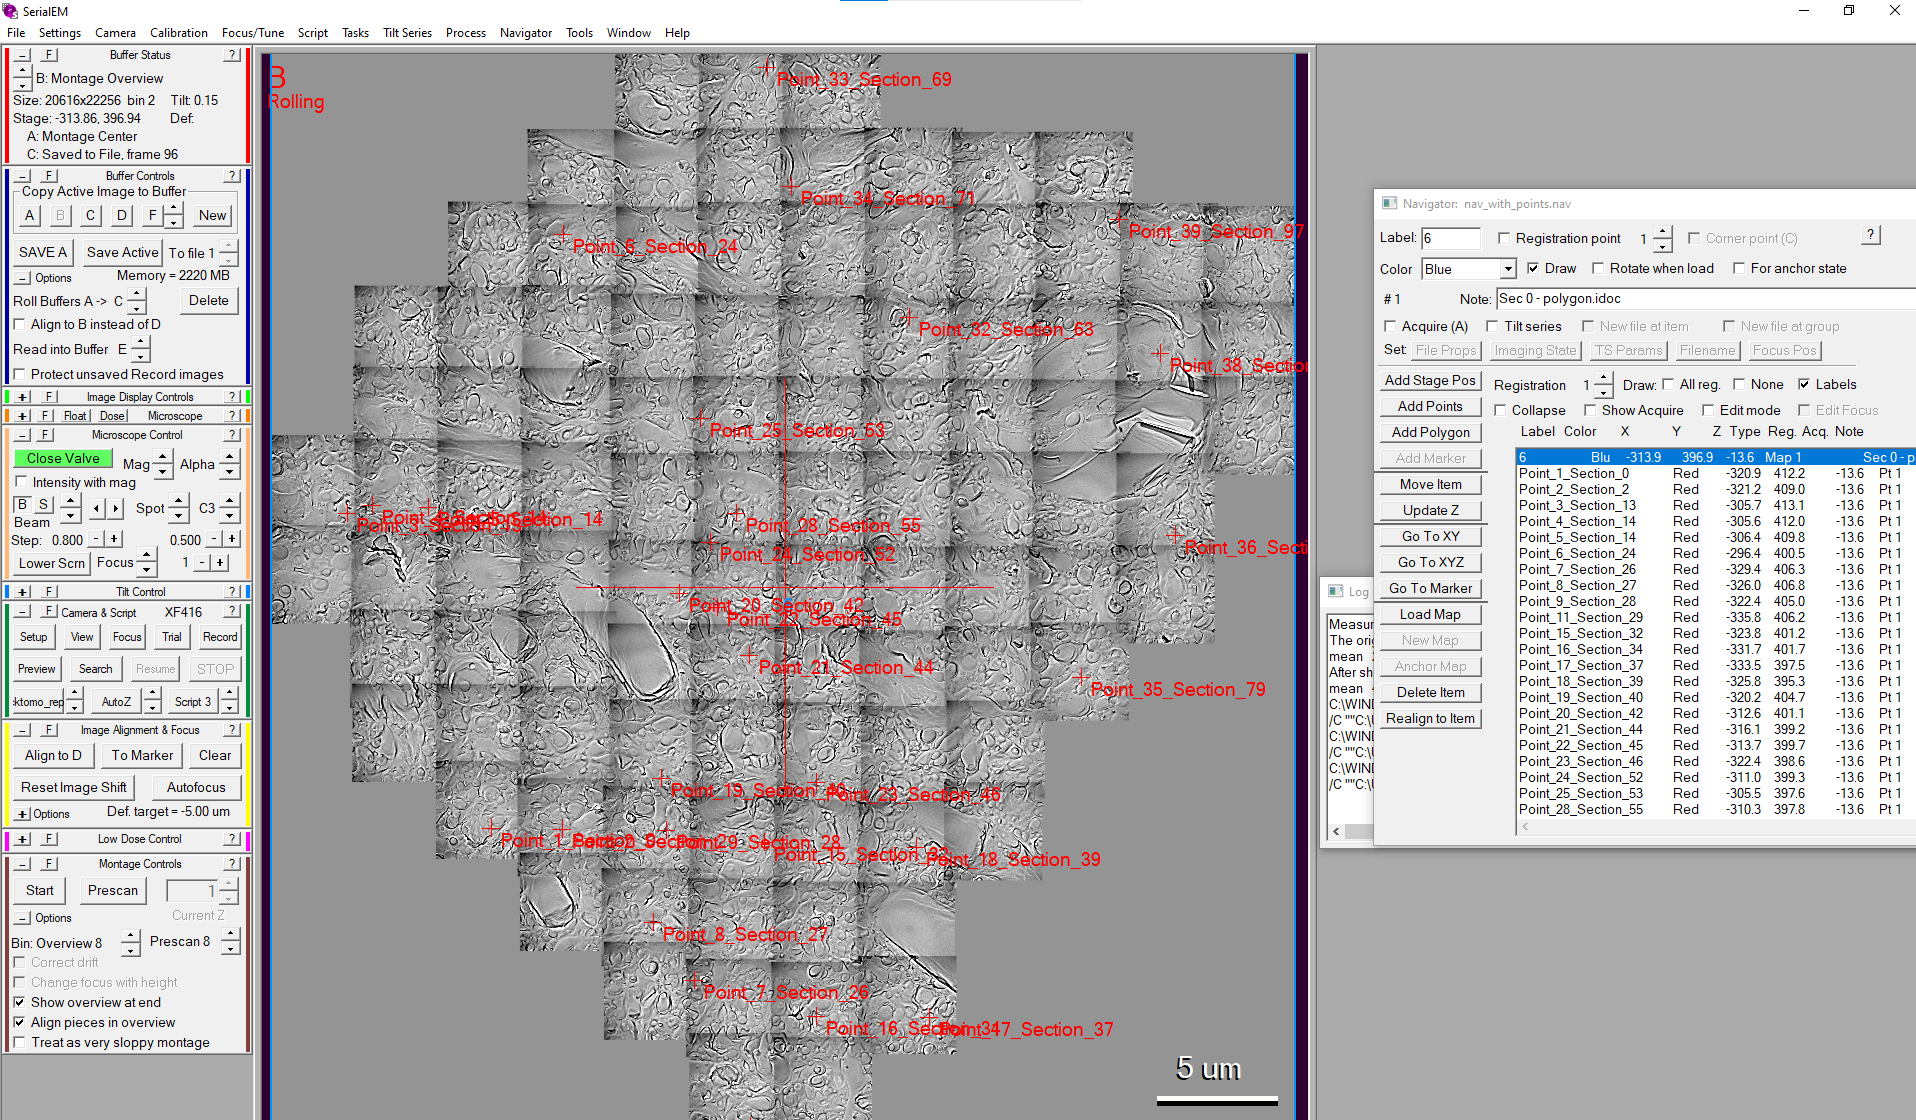
\includegraphics[width=\linewidth]{screenshots/MapWithPoints.png}
\caption{Text}
\end{figure}

\begin{figure}[H]
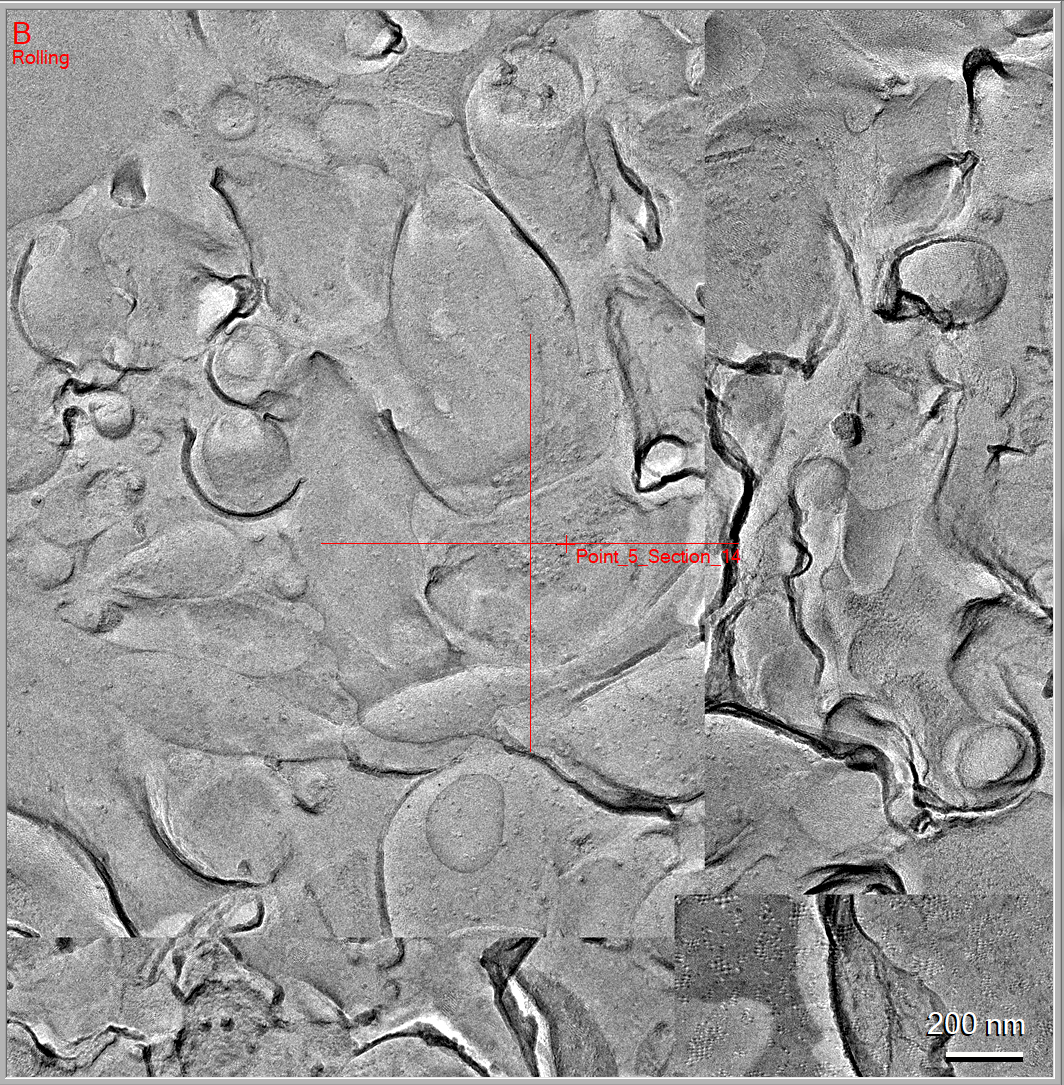
\includegraphics[width=\linewidth]{screenshots/MapWithPointZoom.png}
\caption{Text}
\end{figure}

\section{Tilt Series of the Synapse}

\begin{figure}[H]
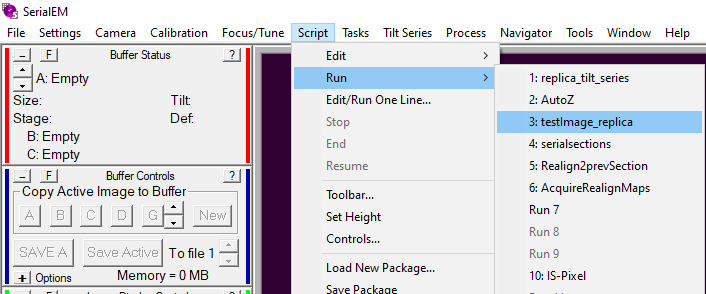
\includegraphics[width=\linewidth]{screenshots/Script_Run.png}
\caption{Text}
\end{figure}

\begin{figure}[H]
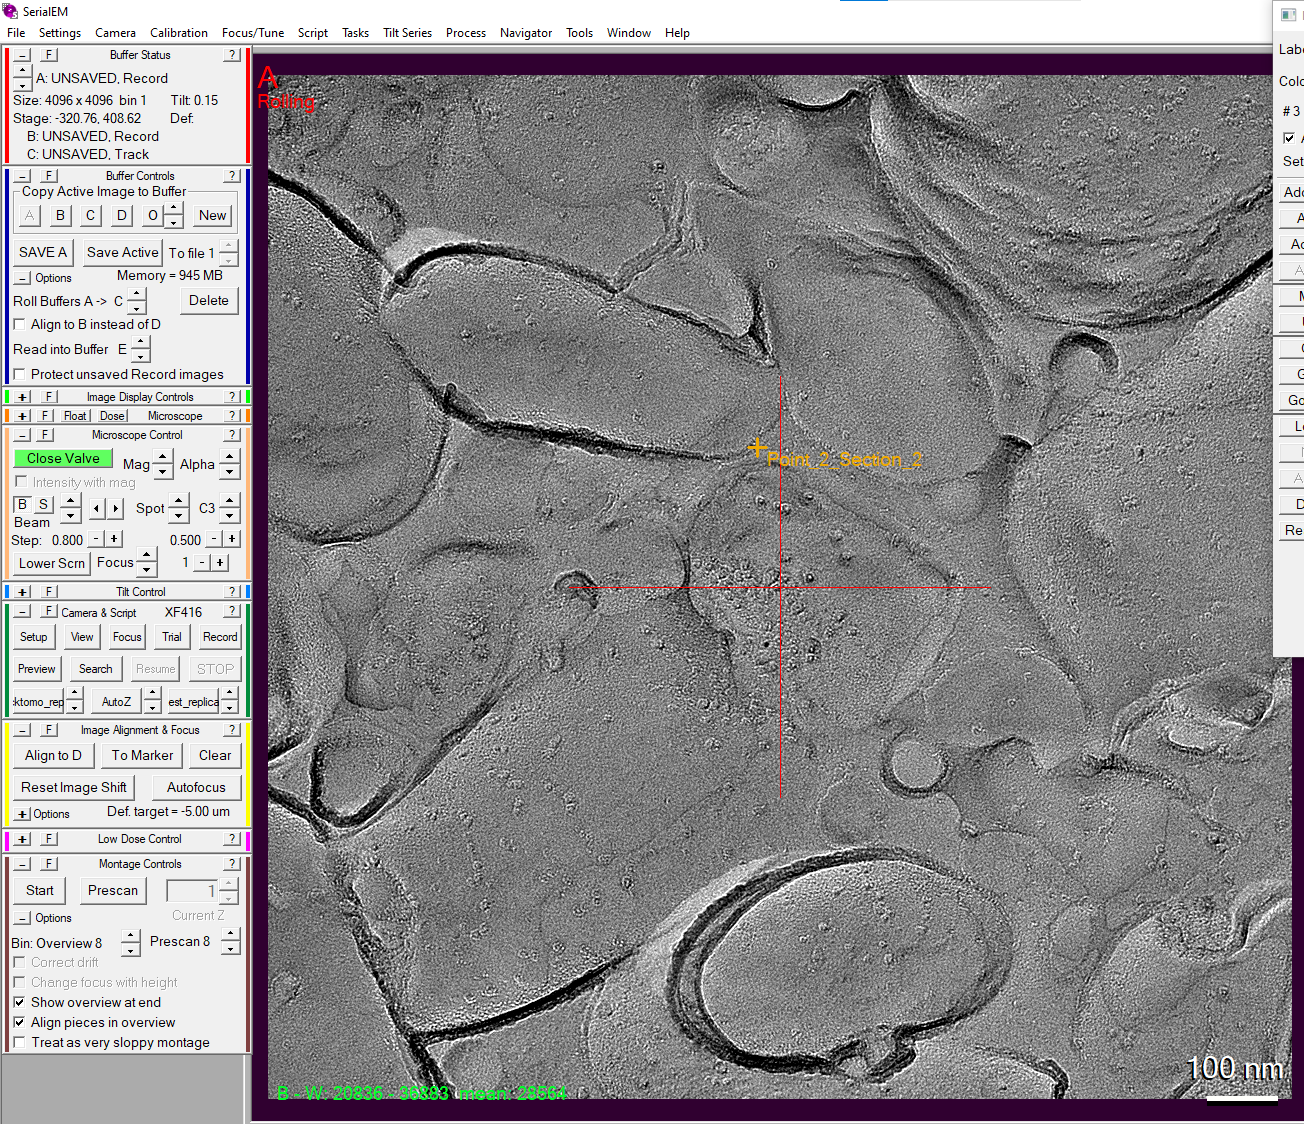
\includegraphics[width=\linewidth]{screenshots/SynapseInCenter.png}
\caption{Text}
\end{figure}

\begin{figure}[H]
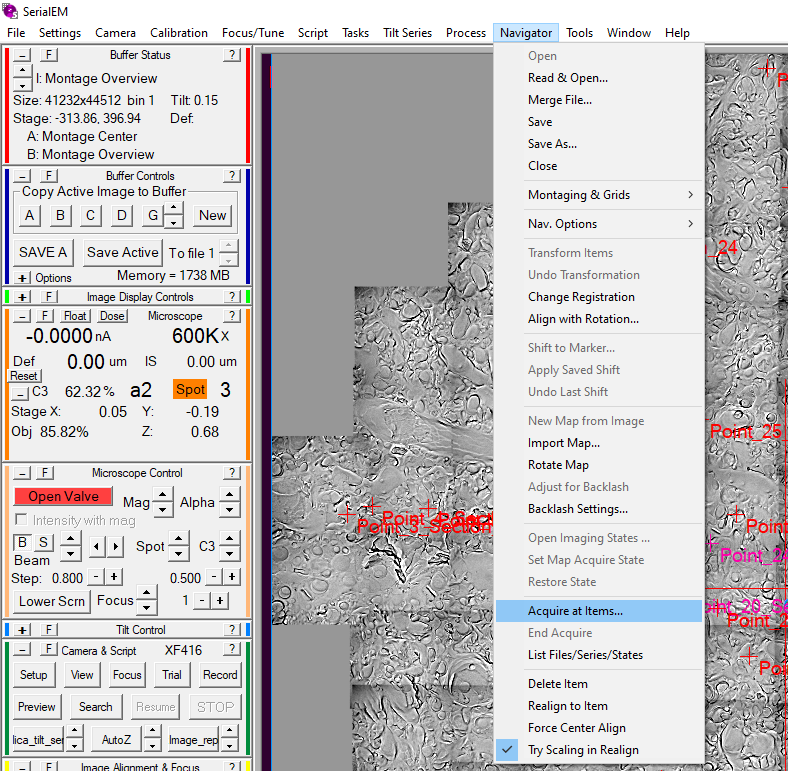
\includegraphics[width=\linewidth]{screenshots/AcquireAtItems.png}
\caption{Text}
\end{figure}

\begin{figure}[H]
\includegraphics[width=\linewidth]{screenshots/AcquireAtItems2.png}
\caption{Text}
\end{figure}

\section{Troubleshooting}

\subsection{Reopen Image}
\begin{figure}[H]
\includegraphics[width=\linewidth]{screenshots/OpenOld.png}
\caption{Text}
\end{figure}

\begin{figure}[H]
\includegraphics[width=\linewidth]{screenshots/Read.png}
\caption{Text}
\end{figure}

\begin{figure}[H]
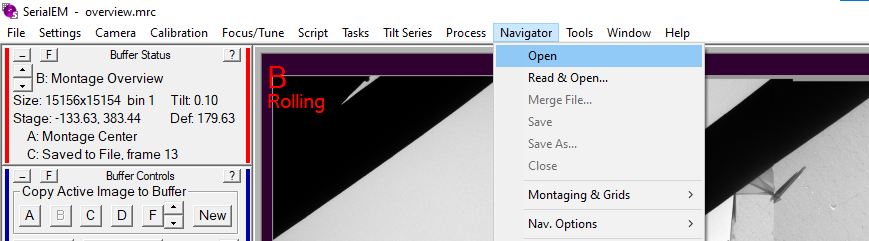
\includegraphics[width=\linewidth]{screenshots/OpenNavigator.png}
\caption{Text}
\end{figure}

Save and rerun tools

\subsection{Synapse not in the center}

\begin{figure}[H]
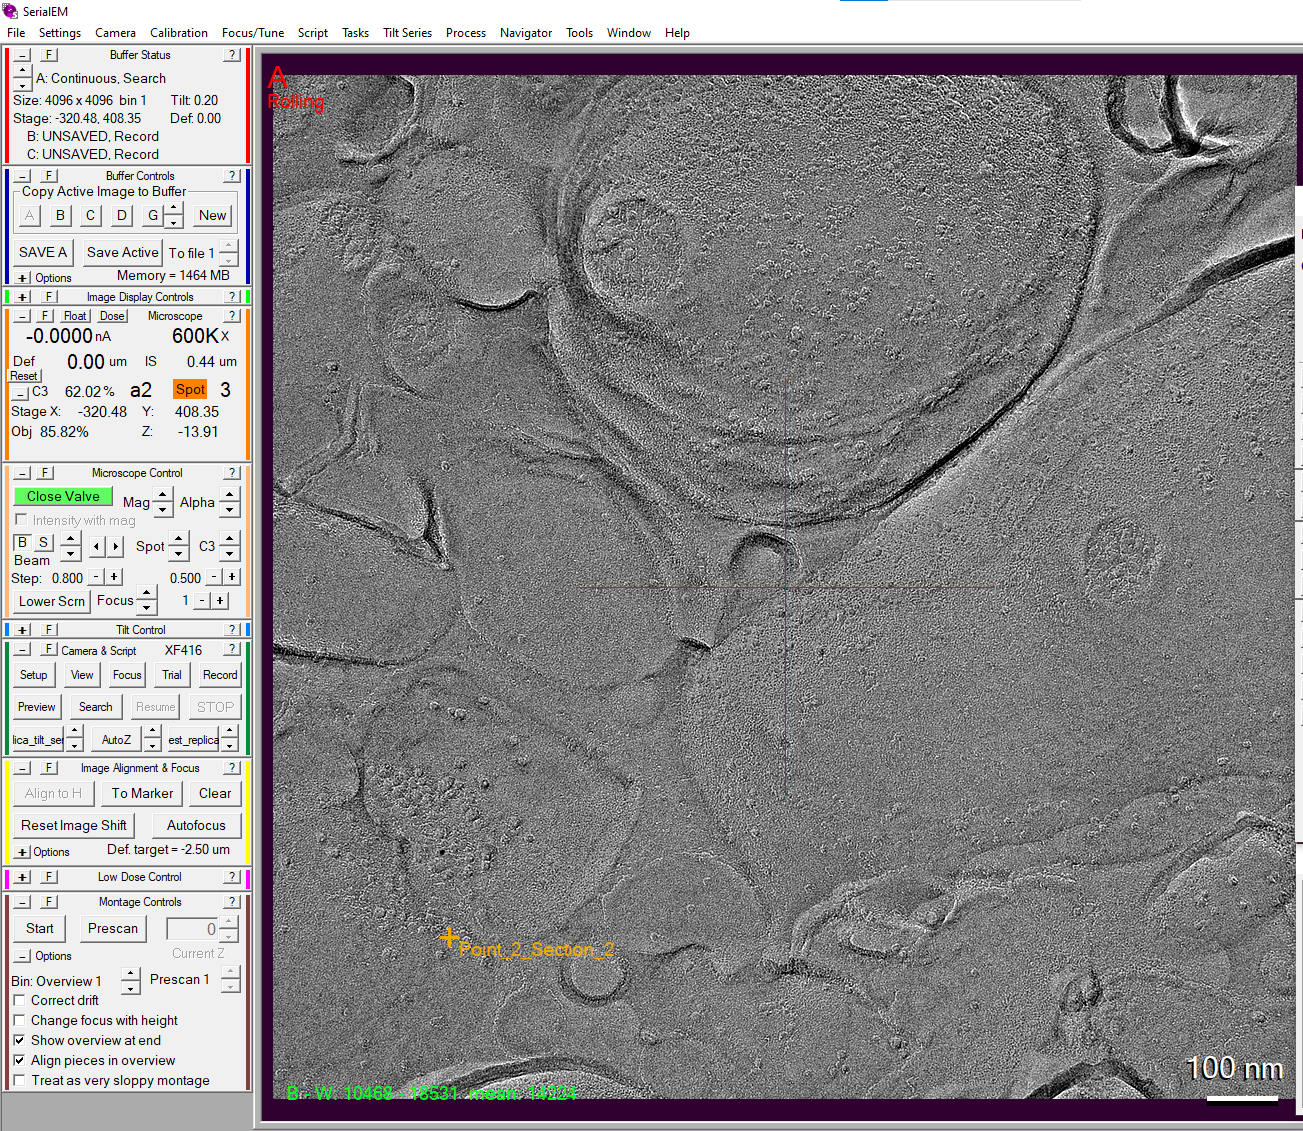
\includegraphics[width=\linewidth]{screenshots/SynapseNotInCenter.png}
\caption{Text}
\end{figure}

Go to map magnification, click realign to item in navigator

\begin{figure}[H]
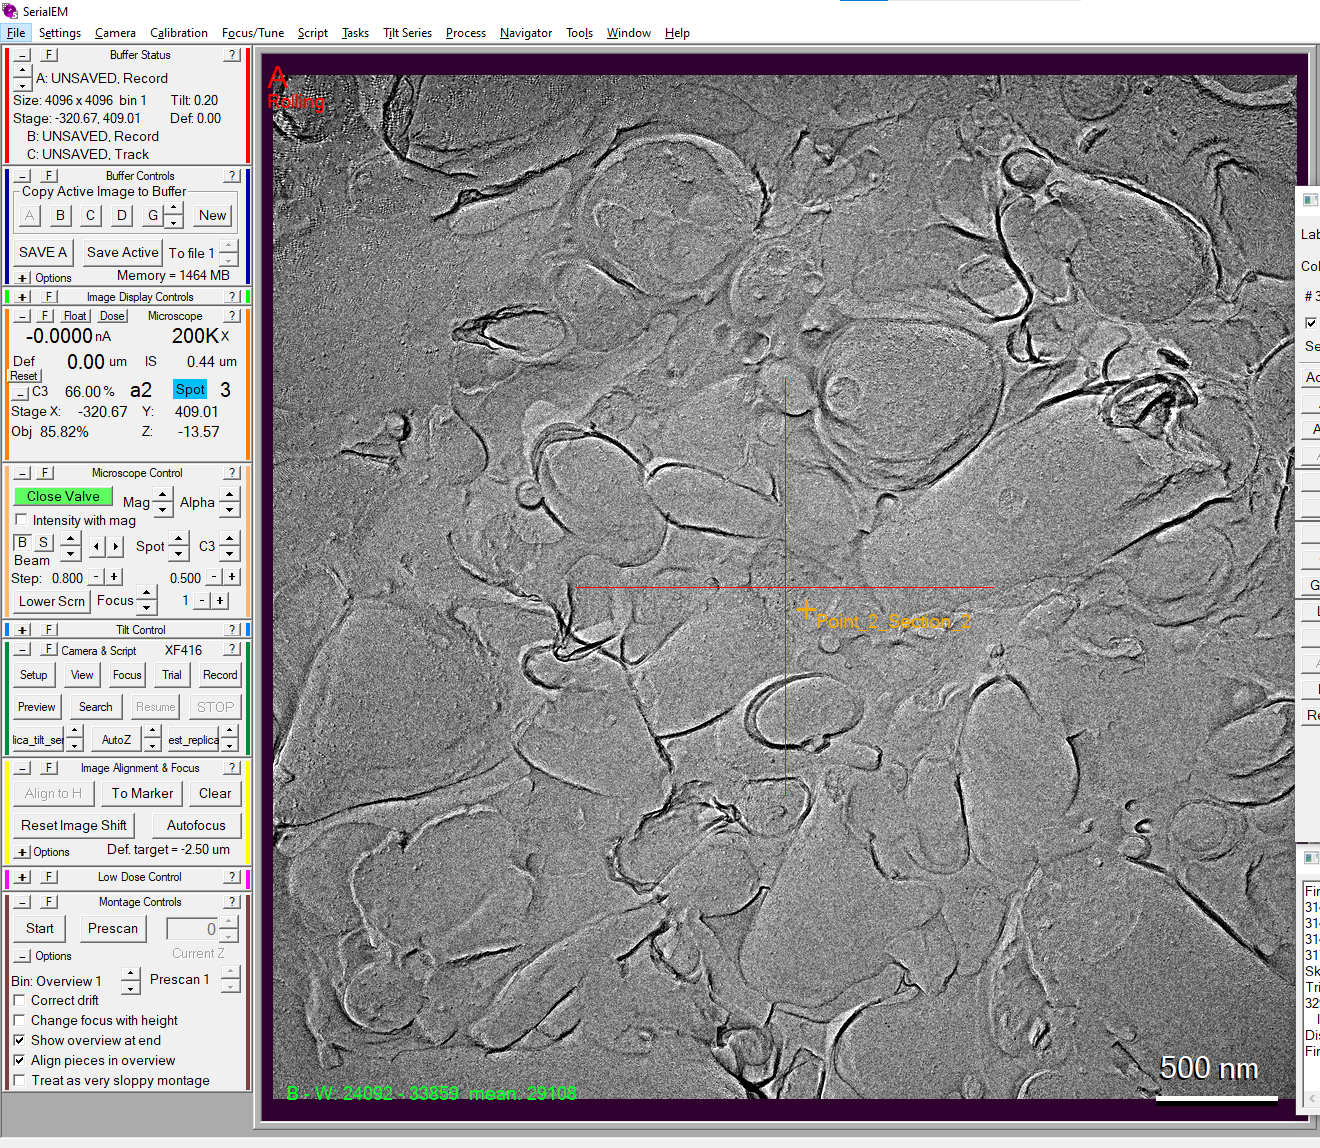
\includegraphics[width=\linewidth]{screenshots/RealignedToItem.png}
\caption{Text}
\end{figure}

\begin{figure}[H]
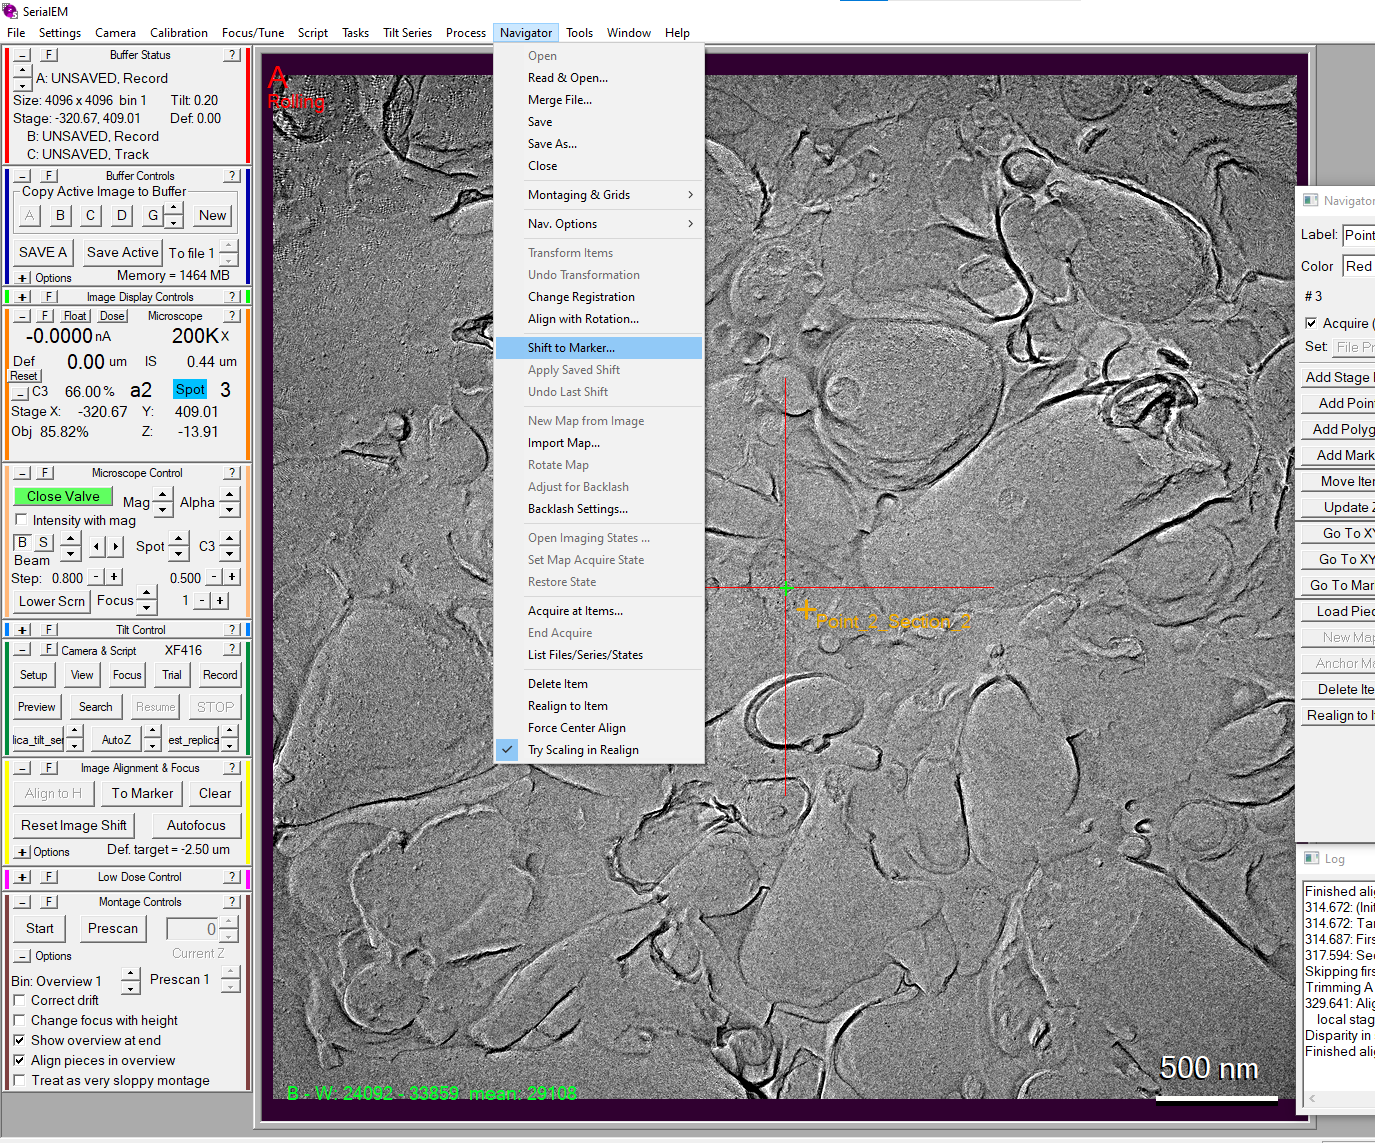
\includegraphics[width=\linewidth]{screenshots/ShiftToMarkerMap.png}
\caption{Text}
\end{figure}

\begin{figure}[H]
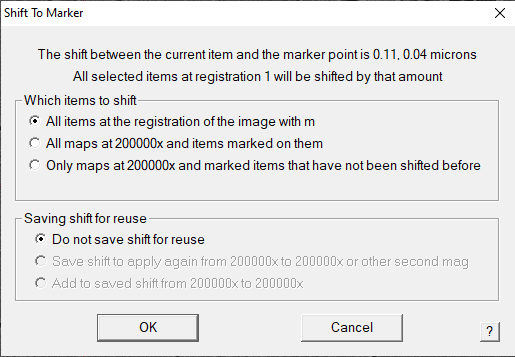
\includegraphics[width=\linewidth]{screenshots/ShiftToMarkerMapMenu.png}
\caption{Text}
\end{figure}

Then go to target Mag

\begin{figure}[H]
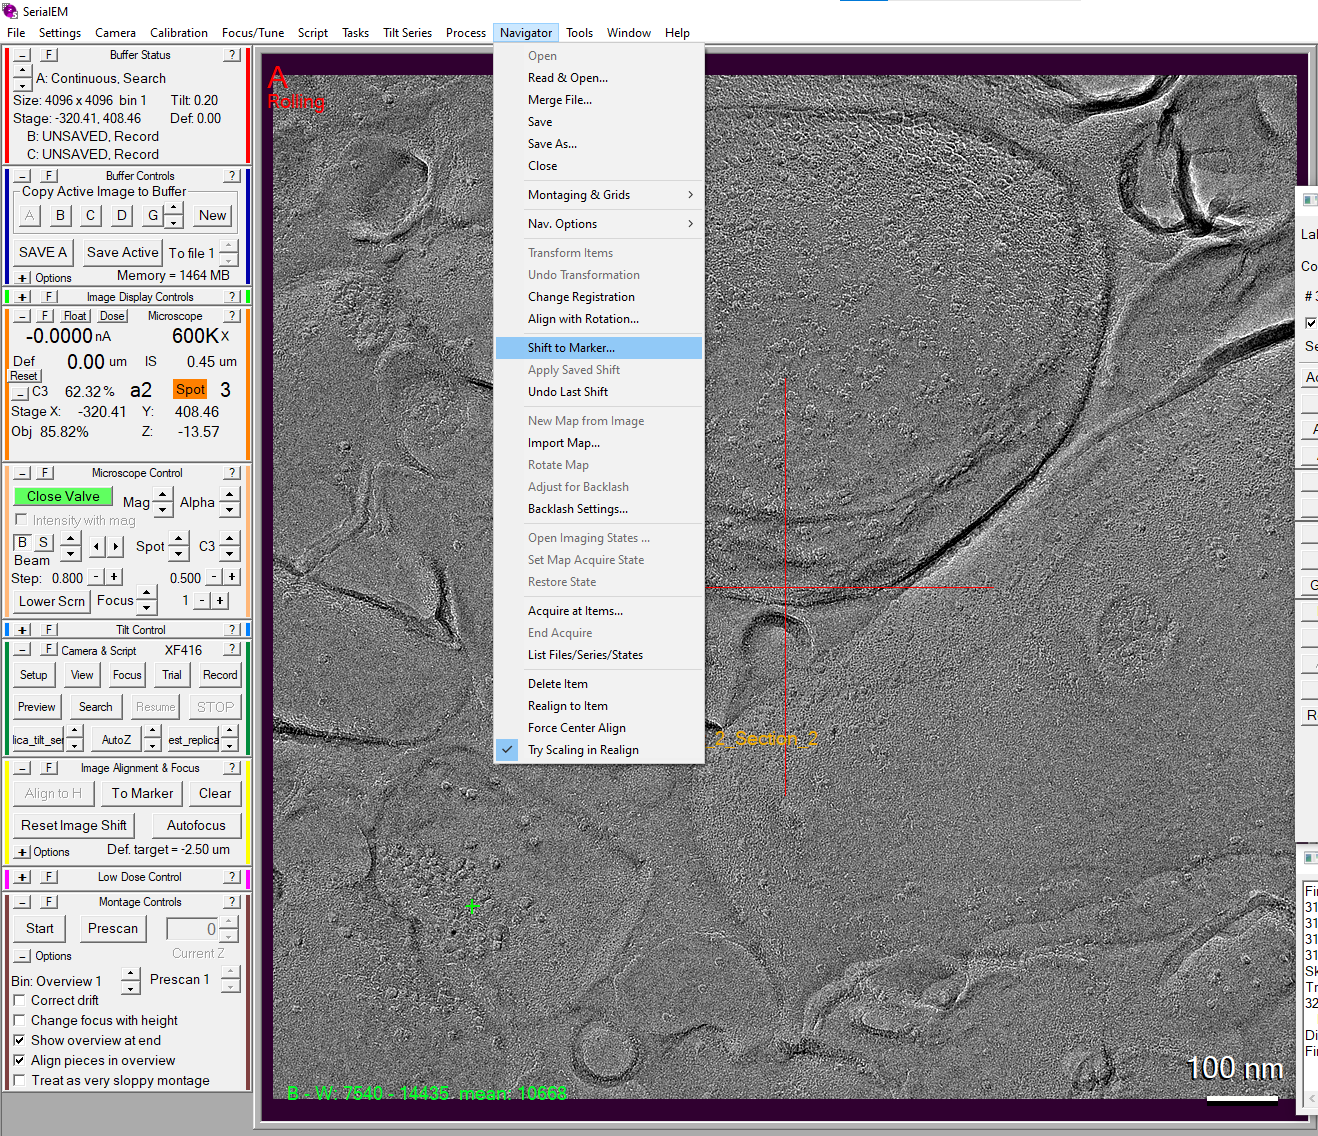
\includegraphics[width=\linewidth]{screenshots/ShiftToMarkerZoom.png}
\caption{Text}
\end{figure}

\begin{figure}[H]
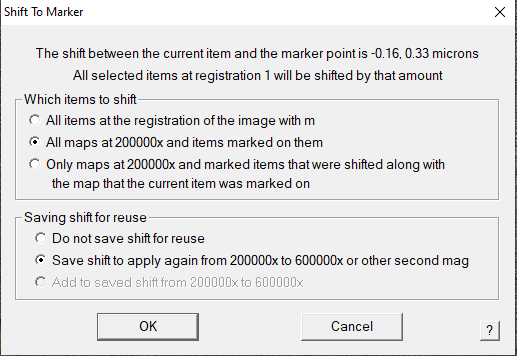
\includegraphics[width=\linewidth]{screenshots/ShiftToMarkerZoomMenu.png}
\caption{Text}
\end{figure}


\end{document}
